\documentclass[aps,pra,12pt,nofootinbib,superscriptaddress,longbibliography,showpacs]{revtex4-1}

\usepackage[utf8]{inputenc}
\usepackage[T1]{fontenc}
\usepackage[english]{babel}  % english language

\usepackage{amssymb,amsmath,amsfonts,amsthm}
\usepackage{mathtools}
\usepackage{verbatim}
\usepackage{enumerate}
%\usepackage{tensor}
\usepackage{fancyhdr}
\pagestyle{fancy}
\usepackage{graphicx}
\graphicspath{{pics/}}
\usepackage{hyperref}
\usepackage{bbm}


\newcommand{\bydef}{\stackrel{\mathrm{def}}{=}}
\renewcommand{\baselinestretch}{1}  % cancels any possible double spacing

\usepackage{color}
%Some shortcuts added for edits
\definecolor{dred}{rgb}{.8,0.2,.2}
\definecolor{ddred}{rgb}{.8,0.5,.5}
\definecolor{dblue}{rgb}{.2,0.2,.8}
% suggested change
\newcommand{\add}[1]{\textcolor{dred}{*** #1 ***}} 
% suggested to remove
\newcommand{\out}[1]{\textcolor{ddred}{\textbf{[}\emph{#1}\textbf{]}}}
% comment or remark
\newcommand{\yo}[1]{\textcolor{dblue}{\textbf{[}#1\textbf{]}}}
\newcommand{\todo}[1]{\textbf{\underline{\textcolor{dblue}{\textbf{[}#1\textbf{]}}}}}

\theoremstyle{plain}
\newtheorem{theorem}{Theorem}   %[section]
\newtheorem{proposition}[theorem]{Proposition}
\newtheorem{lemma}[theorem]{Lemma}
\newtheorem{corollary}[theorem]{Corollary}

\theoremstyle{definition}
\newtheorem{definition}[theorem]{Definition}
\newtheorem{example}[theorem]{Example}
\newtheorem{remark}[theorem]{Remark}

% bra and ket: 
\newcommand{\bra}[1]{\mbox{$\langle #1|$}}
\newcommand{\ket}[1]{\ensuremath{|#1\rangle}}
\newcommand{\braket}[2]{\mbox{$\langle #1|#2\rangle$}}
\newcommand{\ketbra}[2]{\mbox{$|#1\rangle\langle #2|$}}
\newcommand{\iprod}[2]{\ensuremath{\langle #1,#2 \rangle}}

\newcommand{\gate}[1]{\ensuremath{\text{\sc #1}}}
\newcommand{\CCOPY}[1][]{\ensuremath{\gate{COPY}_{#1}}}

\newcommand{\comm}[2]{\ensuremath{\left[#1, #2\right]}}

\newcommand{\eq}{\Leftrightarrow}

\DeclareMathOperator{\Tr}{Tr}
\DeclareMathOperator{\Real}{Re}
\DeclareMathOperator{\Imag}{Im}
\DeclareMathOperator{\Span}{span}
\DeclareMathOperator{\diag}{diag}
\DeclareMathOperator{\Aut}{Aut} % automorphism group
\DeclareMathOperator{\End}{End} % set of endomorphisms

\newcommand{\projector}[1]{\mbox{$|#1\rangle\langle #1|$}}

\newcommand{\x}{\mathbf{x}}
\newcommand{\y}{\mathbf{y}}

\newcommand{\hprod}{\odot}

\newcommand{\I}{\openone}     % identity operator
\newcommand{\R}{{\mathbb R}}  % real numbers
\newcommand{\CC}{{\mathbb C}}  % complex numbers
\newcommand{\hilb}[1]{\ensuremath{\mathcal{#1}}} % Hilbert space
\newcommand{\swap}{{\sf{SWAP}}}
\newcommand{\ie}{i.e.}

% defines logic function names, to look nice 
\newcommand{\be}{\begin{equation}}
\newcommand{\ee}{\end{equation}}

\newcommand{\Figref}[1]{Figure \ref{#1}}

% Quantum communication, Formalism

\def\thesection{%
\arabic{section}}%
\def\thesubsection{%
\arabic{subsection}}%
\def\thesubsubsection{%
\arabic{subsubsection}}%
\def\theparagraph{%
\arabic{paragraph}}%
\def\thesubparagraph{%
\theparagraph.\arabic{subparagraph}}%
\setcounter{secnumdepth}{5}%

% please leave these here 


% fonts 
\def\1#1{{\bf #1}}
\def\2#1{{\cal #1}}
\def\7#1{{\mathbb #1}}


%-------------------------------------------
% Tomi's stuff
%-------------------------------------------

% Fractions
\newcommand{\half}{\mbox{$\textstyle \frac{1}{2}$}}
\newcommand{\quarter}{\mbox{$\textstyle \frac{1}{4}$}}

% Dirac notation
%\newcommand{\ket}[1]{\left | \, #1 \right \rangle}
\newcommand{\kets}[1]{ | \, #1 \rangle}
%\newcommand{\bra}[1]{\left \langle #1 \, \right |}
\newcommand{\bras}[1]{ \langle #1 \, \right}
%\newcommand{\braket}[2]{\left\langle\, #1\,|\,#2\,\right\rangle}
\newcommand{\brakets}[2]{\langle\, #1\,|\,#2\,\rangle}
\newcommand{\bracket}[3]{\left\langle #1 \left| #2 \right| #3 \right\rangle}
\newcommand{\brackets}[3]{\langle #1 | #2 | #3 \rangle}
\newcommand{\proj}[1]{\ket{#1}\bra{#1}}
\newcommand{\av}[1]{\langle #1\rangle}
\newcommand{\outprod}[2]{\ket{#1}\bra{#2}}

% Common operators
\newcommand{\tr}{\textrm{tr}}
%\newcommand{\Tr}{\mathrm{Tr}}
\newcommand{\od}[2]{\frac{\mathrm{d} #1}{\mathrm{d} #2}}
\newcommand{\pd}[2]{\frac{\partial #1}{\partial #2}}
\newcommand{\dt}[1]{\frac{\partial #1}{\partial t}}

% Second quantisation
\newcommand{\an}[1]{\hat{#1}}
\newcommand{\cre}[1]{\hat{#1}^\dag}
\newcommand{\vac}{\ket{\textrm{vac}}}

% Other quantum
\newcommand{\cc}{\textrm{c.c.}}

% Common letters
%\newcommand{\ee}{\mathrm{e}}
%\newcommand{\ii}{\mathrm{i}}
%\newcommand{\dd}{\mathrm{d}}
\newcommand{\identity}{\mathbbm{1}}

% Common symbols
\newcommand{\up}{\uparrow}
\newcommand{\down}{\downarrow}

\renewcommand{\Re}{\mathfrak{Re}}
\renewcommand{\Im}{\mathfrak{Im}}

% Letters in different styles

\newcommand{\AAA}{\mathbf{A}}
\renewcommand{\AA}{\mathcal{A}}
\newcommand{\aaa}{\mathbf{a}}
\renewcommand{\aa}{\mathrm{a}}
\newcommand{\BBB}{\mathbf{B}}
\newcommand{\BB}{\mathcal{B}}
\newcommand{\bbb}{\mathbf{b}}
\newcommand{\bb}{\mathrm{b}}
\newcommand{\CCCC}{\mathbf{C}}
\newcommand{\CCC}{\mathcal{C}}
\newcommand{\ccc}{\mathbf{c}}
\renewcommand{\cc}{\mathrm{c}}
\newcommand{\DDD}{\mathbf{D}}
\newcommand{\DD}{\mathcal{D}}
\newcommand{\ddd}{\mathbf{d}}
\newcommand{\dd}{\mathrm{d}}
\newcommand{\EEE}{\mathbf{E}}
\newcommand{\EE}{\mathcal{E}}
\newcommand{\eee}{\mathrm{e}}
%\newcommand{\ee}{\mathrm{e}}
\newcommand{\FFF}{\mathbf{F}}
\newcommand{\FF}{\mathcal{F}}
\newcommand{\fff}{\mathbf{f}}
\newcommand{\ff}{\mathrm{f}}
\newcommand{\GGG}{\mathbf{G}}
\newcommand{\GG}{\mathcal{G}}
\renewcommand{\ggg}{\mathbf{g}}
\renewcommand{\gg}{\mathrm{g}}
\newcommand{\HHH}{\mathbf{H}}
\newcommand{\HH}{\mathcal{H}}
\newcommand{\hhh}{\mathbf{h}}
\newcommand{\hh}{\mathrm{h}}
\newcommand{\III}{\mathbf{I}}
\newcommand{\II}{\mathcal{I}}
\newcommand{\iii}{\mathbf{i}}
\newcommand{\ii}{\mathrm{i}}
\newcommand{\JJJ}{\mathbf{J}}
\newcommand{\JJ}{\mathcal{J}}
\newcommand{\jjj}{\mathbf{j}}
\newcommand{\jj}{\mathrm{j}}
\newcommand{\KKK}{\mathbf{K}}
\newcommand{\KK}{\mathcal{K}}
\newcommand{\kkk}{\mathbf{k}}
\newcommand{\kk}{\mathrm{k}}
\newcommand{\LLL}{\mathbf{L}}
\newcommand{\LL}{\mathcal{L}}
\renewcommand{\lll}{\mathbf{l}}
\renewcommand{\ll}{\mathrm{l}}
\newcommand{\MMM}{\mathbf{M}}
\newcommand{\MM}{\mathcal{M}}
\newcommand{\mmm}{\mathbf{m}}
\newcommand{\mm}{\mathrm{m}}
\newcommand{\NNN}{\mathbf{N}}
\newcommand{\NN}{\mathcal{N}}
\newcommand{\nnn}{\mathbf{n}}
\newcommand{\nn}{\mathrm{n}}
\newcommand{\OOO}{\mathbf{O}}
\newcommand{\OO}{\mathcal{O}}
\newcommand{\ooo}{\mathbf{o}}
\newcommand{\oo}{\mathrm{o}}
\newcommand{\PPP}{\mathbf{P}}
\newcommand{\PP}{\mathcal{P}}
\newcommand{\ppp}{\mathbf{p}}
\newcommand{\pp}{\mathrm{p}}
\newcommand{\QQQ}{\mathbf{Q}}
\newcommand{\QQ}{\mathcal{Q}}
\newcommand{\qqq}{\mathbf{q}}
\newcommand{\qq}{\mathrm{q}}
\newcommand{\RRR}{\mathbf{R}}
\newcommand{\RR}{\mathcal{R}}
\newcommand{\rrr}{\mathbf{r}}
\newcommand{\rr}{\mathrm{r}}
\newcommand{\SSS}{\mathbf{S}}
\renewcommand{\SS}{\mathcal{S}}
\newcommand{\sss}{\mathbf{s}}
\renewcommand{\ss}{\mathrm{s}}
\newcommand{\TTT}{\mathbf{T}}
\newcommand{\TT}{\mathcal{T}}
\newcommand{\ttt}{\mathbf{t}}
\renewcommand{\tt}{\mathrm{t}}
\newcommand{\UUU}{\mathbf{U}}
\newcommand{\UU}{\mathcal{U}}
\newcommand{\uuu}{\mathbf{u}}
\newcommand{\uu}{\mathrm{u}}
\newcommand{\VVV}{\mathbf{V}}
\newcommand{\VV}{\mathcal{V}}
\newcommand{\vvv}{\mathbf{v}}
\newcommand{\vv}{\mathrm{v}}
\newcommand{\WWW}{\mathbf{W}}
\newcommand{\WW}{\mathcal{W}}
\newcommand{\www}{\mathbf{w}}
\newcommand{\ww}{\mathrm{w}}
\newcommand{\XXX}{\mathbf{X}}
\newcommand{\XX}{\mathcal{X}}
\newcommand{\xxx}{\mathbf{x}}
\newcommand{\xx}{\mathrm{x}}
\newcommand{\YYY}{\mathbf{Y}}
\newcommand{\YY}{\mathcal{Y}}
\newcommand{\yyy}{\mathbf{y}}
\newcommand{\yy}{\mathrm{y}}
\newcommand{\ZZZ}{\mathbf{ZZ}}
\newcommand{\ZZ}{\mathcal{ZZ}}
\newcommand{\zzz}{\mathbf{z}}
\newcommand{\zz}{\mathrm{z}}


% Referencing
\newcommand{\eqr}[1]{Eq.~(\ref{#1})}
\newcommand{\fir}[1]{Fig.~\ref{#1}}
\newcommand{\secr}[1]{Sec.~\ref{#1}}
\newcommand{\apr}[1]{App.~\ref{#1}}
\newcommand{\chr}[1]{Ch.~\ref{#1}}


% kill double space 
\renewcommand{\baselinestretch}{1} 

% Complexity classes 
\newcommand{\NP}{\mathrm{NP}}
\renewcommand{\P}{\mathrm{P}} 

\begin{document}

%\newcommand{\captionfonts}{\small}
%\makeatletter  % Allow the use of @ in command names
%\long\def\@makecaption#1#2{%
%  \vskip\abovecaptionskip
%  \sbox\@tempboxa{{\captionfonts #1: #2}}%
%  \ifdim \wd\@tempboxa >\hsize
%    {\captionfonts #1: #2\par}
%  \else
%    \hbox to\hsize{\hfil\box\@tempboxa\hfil}%
%  \fi
%  \vskip\belowcaptionskip}
%\makeatother   % Cancel the effect of \makeatletter

\title{Chiral Quantum Walks}

\author{Ville Bergholm}
\affiliation{Institute for Scientific Interchange,
Via Alassio 11/c, 10126
Torino, Italy}

\author{Mauro Faccin}
%\email{jacob.biamonte@qubit.org}
\affiliation{Institute for Scientific Interchange,
Via Alassio 11/c, 10126
Torino, Italy} 

\author{Jacob Biamonte}
%\email{jacob.biamonte@qubit.org}
\affiliation{Institute for Scientific Interchange,
Via Alassio 11/c, 10126
Torino, Italy}

\author{Tomi Johnson}
%\email{jacob.biamonte@qubit.org}
\affiliation{Institute for Scientific Interchange,
Via Alassio 11/c, 10126 
Torino, Italy} 
\affiliation{University of Oxford} 

%\author{Sabre Kais?}
%\email{jacob.biamonte@qubit.org}
%\affiliation{Purdue}
%\affiliation{QEERI} 

\author{Seth Lloyd}
\affiliation{MIT, Cambridge USA} 



\begin{abstract}
It was recently found that transition probabilities in typical quantum
walks take the same value when the time
coordinate changes sign from positive to negative.  This subtlety was
then shown to prohibit directional biasing and assert that the
transition rates themselves carry what turned out to be an often
restrictive symmetry.  However, even in unitary dynamics, transition
rate time-symmetry can be broken, thereby enabling directional
biasing, enhancement and suppression of quantum transport.  Here we
extend the theory of these so called ``chiral quantum walks'' by
considering the mathematical structure surrounding this symmetry and
its related properties.  We close with an experimental proposal, which
would represent the first demonstration of a chiral quantum walk
requiring a 3-spin NMR quantum information processor.
\end{abstract} 


\maketitle

\section{vision for the structure} 

Introductory 1 page about. 
\begin{itemize}
 \item Begin explaining standard symmetry vs antilinear symmetry 
 
 \item Description of how such phases enable directional transport (simple figure explaining how the phases send a walker down one side or the other of an odd loop.  Contrasting even and odd loops. 
 
 \item Description of how gauge theory allows one to manipulate network diagrams etc. 
 
 \item Motivating the need for circuits and the motivation for time-independent control 
 
\end{itemize}

Results 1-2 pages. 

\begin{itemize}
 \item Explain the constraints of the definition and how care must be taken to demonstrate the effect experimentally.  
 
 \item The proposed circuit, its theory and some numerics simulation.  Explaining how it can also be first viewed as a trotter step of the prior theory, but how we can adjust the angles in the gates to get perfect transfer.  
 
 \item Explain how the dagger of the circuit etc. can be taken by additional gates which transform the above circuit into a time-reversed one etc. 
 
 \item Some general consequences of the proposed theory.  Connection to matchgates.  
 
\end{itemize}

Concluding remarks and implications of the theory.  1 page about.  

\begin{itemize}
 \item  Analysis and more general statements about the proposed work and its differences, etc. from past approaches. 
 
 \item Prospects for future devices that use this effect.  Including again mentioning that biological systems might actually have phases in their hamiltonians. 
 
\end{itemize}


\section{Comments, TODOs etc.}

\begin{itemize}
\item
(Explicit) symmetry breaking normally means that the system Hamiltonian
almost obeys some symmetry, but a small perturbation term breaks
it. In our case it would be better to say that the Hamiltonians (or
states) either are T-symmetric, or are not T-symmetric.

\item
Gauge group: a Lie group that the Hamiltonian is invariant
under. In our case, is there any difference between local and global
gauge transformations?

\item We have been concerned with the gauge symmetry of the transition amplitudes: here this is only a quasi gauge theory as it is basis dependent.  We have not been considering yet the gauge group of the Hamiltonians.  

\item Justification of why the gate model approach subsumes and extends the Hamiltonian picture in specific ways. You can change from a propagator that does not break time symmetry to one that does using only local Z gates (opening new prospects for the control of energy and information flow).  The gate approach will enable an NMR experiment (other systems would likely be unable to realize the circuit proposed in the draft since it requires 6 two body gates).  In addition, by viewing the hamiltonian induced evolution in terms of a Trotter sequence, and taking a single symmetric time slice, you find the same circuit that we're proposing (though by different means).  Adjusting the angles of the gates (and hence actually making a worse Trotter approximation) increase the transport control.  In other words, you can take one time-slice (a 6 gate circuit) and get optimal directed transport.  So ultimately the gate approach is limited in some ways, but does open up some interesting possibilities, and at the very 
least an experimental demonstration with existing quantum computing hardware.  You can always recover the Hamiltonian from the gate model by considering a Trotter sequence, and of course, the converse is true due to Stone's theorem (in principle though the generators found from inverting a propagator could be complicated).  

\end{itemize}


\section{The main idea} 

In this paper we propose to study the chiral quantum walks, leverging techniques from the quantum circuits language.  Here we are developing a theory of circuits, to understand when these circuits break time symmetry.  To accomplish this goal, we reexamine the basic definitions of time-symmetry breaking and arrive at a more precise understanding.  

The advantage of the circuits approach is that even for simple networks, we see
that the chiral effects play a dominant role.  To examine this effect,
we are proposing 4 experiments.  In the first experiment, we consider
a circuit which does not break time symmetry.  A similarity transform,
given by local operations, shows that this circuit can be transformed
into one which breaks time symmetry.  In both cases, the dagger of the
circuits can be examined experimentally by considering similarity
transforms.

One might think that what we're doing is comparing two gate families, and that we notice different transport properties between these two.  However, our results are more general than this.  There is a theory of gauge transforms, that shows that in many cases, the chiral and the symmetry Hamiltonians can not be distinguished.  Time-symmetry breaking turns out to be intimately connected to the geometry of the network on which a Hamiltonian acts.  

\section{Tomi's point of view}
\subsection{Motivation}
The vast majority of studies on quantum walks have been restricted to walks in which the single particle internode hopping amplitudes are real. Coupled with the requirement of Hermiticity, this prohibits any directedness of the quantum walk. The probability of a walker moving to node $n$ having started in node $m$ is the same as moving to $m$ from $n$; the walk is unbiased and undirected. Equivalently, the probabilities of moving from one node to another while going forwards and backwards in time are identical. Hence these walks are called time-inversion symmetric.

However, in a chiral quantum walk the single particle internode hopping amplitudes may be complex. As such, when time is inverted the interference of the walker's paths is changed in a non-trivial way, providing a means of breaking the internode transition probability time-inversion symmetry. This is by no means guaranteed, however, and whether or not the symmetry is broken --- as well as to what extent --- depends delicately on the relationship between the phases of the hopping amplitudes and the geometry of the walk. It is left to this work, therefore, to study the conditions for the biasing of a quantum walk and introduce a measure for the degree of this biasing. 

Our study considers unitary walks on complex networks, with non-zero phases on the hopping amplitudes. This contrasts with dynamics considered in condensed matter, which by default include strong dissipative processes. For example, in a dissipative walk on a line, the application of phases to the nearest-neighbor hopping amplitudes is equivalent to an applied voltage and results in a biased walk. However, in the corresponding unitary system, without dissipation, time-inversion symmetry is unbroken. This work also extends the analysis beyond a restrictive lattice structure, where phases are created uniformly across the system, to consider the possibilities arising from local control over phases resulting in a heterogenous walk.

At its heart, this is therefore a work that shows how to introduce or enhance directedness and biasing in quantum dynamics. This has obvious implications in the design of quantum mechanical wires for energy or particle transport. Another application arises in the use of quantum walks in classifying a directed complex network, e.g., to rank nodes, which requires a means of reflecting the directedness of the network in the quantum walk.

\subsection{Identifying time-inversion symmetry breaking}
The definition of time-inversion symmetry breaking is that the internode transition probabilities should be the same when going forwards or backwards in time, i.e.,
\begin{align}
\label{eq:def1}
| \bra{n} \eee^{-\ii H t} \ket{m} |^2 = | \bra{n} \eee^{\ii H t} \ket{m} |^2 ,
\end{align}
for all $n$ and $m$. By taking the conjugate within the absolute value on the right hand side, \eqr{eq:def1} is equivalent to
\begin{align}
\label{eq:def2}
| \bra{n} \eee^{-\ii H t} \ket{m} |^2 = | \bra{m} \eee^{-\ii H t} \ket{n} |^2 .
\end{align}
This is the condition that the walk is unbiased; the probability of moving to node $n$ having started in node $m$ is the same as moving to $m$ from $n$.

It is clear that if the there are no phases on the hopping amplitudes, i.e., $\bra{n} H \ket{m}$ is real, then time-inversion symmetry is never broken. This follows from the fact that in this case the conjugate of $\bra{n} \eee^{-\ii H t} \ket{m}$ is $\bra{n} \eee^{\ii H t} \ket{m}$, thus \eqr{eq:def1} is satisfied.

To break time-inversion symmetry thus necessitates a chiral walk, with complex amplitudes $\bra{n} H \ket{m}$. The question we must address is in what cases this symmetry is broken. To begin to answer this question, we rewrite \eqr{eq:def1} as $f(t) = 0$ for all $t$, where
\begin{align}
\label{eq:def3}
f(t) = | \bra{n} \eee^{-\ii H t} \ket{m} |^2 - | \bra{n} \eee^{\ii H t} \ket{m} |^2 .
\end{align}
We then expand the square of the absolute values and Taylor expand the exponentials to obtain
\begin{subequations}
\label{eq:def4}
\begin{align}
f(t) &=  \bra{n} \eee^{-\ii H t} \ket{m} \bra{m} \eee^{\ii H t} \ket{n} -  \bra{n} \eee^{\ii H t} \ket{m} \bra{m} \eee^{- \ii H t} \ket{n}  \\
&= \sum_{k=0}^\infty \sum_{l=0}^\infty \frac{(-\ii t)^k (\ii t)^l}{k! l!} \left( \bra{n} H^k \ket{m} \bra{m} H^l \ket{n} -  \bra{n} H^l \ket{m} \bra{m} H^k \ket{n} \right) .
\end{align}
\end{subequations}
With a slight relabelling this becomes
\begin{subequations}
\label{eq:def4}
\begin{align}
f(t) &= \sum_{k=0}^\infty \sum_{l=0}^\infty \frac{(-1)^k (\ii t)^{k+l}}{k! l!} \left( \bra{n} H^k \ket{m} \bra{m} H^l \ket{n} -  \bra{n} H^l \ket{m} \bra{m} H^k \ket{n} \right)  \\
&=  \frac{1}{2} \sum_{M=0 }^\infty (\ii t)^{M} \sum_{k=0}^{M} \frac{ (-1)^k - (-1)^{M-k}}{k! (M-k)!}  \left( \bra{n} H^k \ket{m} \bra{m} H^{M-k} \ket{n} -  \bra{n} H^{M-k}\ket{m} \bra{m} H^k \ket{n} \right) .
\end{align}
\end{subequations}
Time-inversion symmetry is equivalent to $f(t) = 0$ for all $t$, and this is equivalent to requiring that the coefficient for each power of $t$ disappears separately (this can be thought of as demanding that all derivatives of $f(t)$ vanish), i.e.,
\begin{align}
\label{eq:def5}
\sum_{k=0 }^{M} \frac{ (-1)^k - (-1)^{M-k}}{k! (M-k)!}  \left( \bra{n} H^k \ket{m} \bra{m} H^{M-k} \ket{n} -  \bra{n} H^{M-k} \ket{m} \bra{m} H^k \ket{n} \right)  = 0 ,
\end{align}
for all $m$, $n$ and $M$.
This shows that time-symmetry corresponds to a Hamiltonian satisfying algebraic condition on its elements in some orthonormal basis\footnote{Note for us: This equation captures all conditions; time inversion symmetry at all times and the fact that the dynamics is generated by a Hamiltonian. It is of quite a nice form, e.g., it doesn't say ``there exists some phase matrix such that when its Hadamard product with the unitary the transpose is obtained, and this is true for all times t''.}.

Before we continue, let us simplify this expression somewhat by identifying parts that are trivially zero. First, for all even $M$ we have $(-1)^k - (-1)^{M-k} = 0$, while for odd $M$ we have $(-1)^k - (-1)^{M-k} = 2 (-1)^k$. Therefore we only need to consider odd $M$. Second, the first term on the right hand side of \eqr{eq:def5} for $k = l$ is identical to the second term form $k = M -l$, while the terms for $k = 0$ and $k = M$ are zero. Therefore we only need to consider either one term or the other. This means that the time-symmetric condition becomes
\begin{align}
\label{eq:def6}
  \sum_{k=1 }^{M-1} (-1)^k \frac{   \bra{n} H^{M-k} \ket{m} \bra{m} H^k \ket{n}}{k! (M-k)!}   = 0 ,
\end{align}
for all $n$, $m$ and odd $M$. 

\subsubsection{Loops}
\yo{The below could probably be written in terms of path sums, the discrete analogue of path integrals. We can discuss what the best presentation style could be.}
From \eqr{eq:def1} there is already a clear interpretation of this time-symmetry condition in terms of the magnitude of the summed amplitudes corresponding to walks from $n$ to $m$. Equation (\ref{eq:def6}) allows an interpretation in terms of walks from $n$ back to itself. The amplitude associated with such a loop is
\begin{subequations}
\label{eq:loopamp}
\begin{align}
A(n,t) &= \bra{n} \eee^{-\ii H t} \ket{n} \\
&= \bra{n} \left( \mathbbm{1} + \ii H t + \frac{\ii^2 H^2 t^2}{2} + \cdots + \frac{\ii^M H^M t^M}{M!} + \cdots  \right) \ket{n}.
\end{align}
\end{subequations}
We focus on the part of this corresponding to $M$ transitions
\begin{align}
\label{eq:Mloopamp}
A(n,M,t) = \frac{ \ii^M t^M}{M!} \bra{n} H^M \ket{n}.
\end{align}
Further, we pick out the part of the amplitude corresponding to a loop that goes through another node $m$. This itself breaks down into contributions corresponding to the arrival at node $m$ after $k$ transitions
\begin{subequations}
\label{eq:mMloopamp}
\begin{align}
A(n,m,M,t) &= \sum_{k=0}^M A(n,m,k,M,t) , \\
A(n,m,k,M,t) &=\frac{ \ii^M t^{M} }{ M!} \frac{ \bra{n} H^{M-k} \ket{m} \bra{m}  H^k \ket{n} }{k! (M-k)! }  .
\end{align}
\end{subequations}

This provides an interpretation of \eqr{eq:def6} in terms of the amplitude corresponding to loops, since the time-inversion symmetric condition may now be written as
\begin{align}
\label{eq:def7}
  \sum_{k=1 }^{M-1} (-1)^k  A(n,m,k,M,t)   = 0 ,
\end{align}
for all $n$, $m$ and odd $M$ (and for any $t$). 

We can make two inferences from this. First, breaking time-inversion symmetry comes down to breaking a symmetry in the loops of odd length. If no loops of odd length exist, e.g., for walks on a bipartite graph (this includes all square lattices), then time-symmetry cannot be broken. Second, loops of odd length do not include loops that leave and return along the same path. Therefore only loops that enclose a non-zero area contribute. If there are no such loops, then time-inversion symmetry is always obeyed.

The argument above is very general and the states $\ket{n}$ need not be the node basis, but could be any orthonormal basis. This provides a nice no-go for asymmetric transport and shows how the geometry of configuration space effects transport properties, regardless of the parameters; traingular and square lattices have fundamentally different transport properites.

Note also that there unless our Hamiltonian is equivalent to one with zero along the diagonal, there is an important distinction between the graph in physical space (which has no self-loops) and the graph in configurational space (which may have self-loops). Our discussion here is in configuration space and therefore self-loops will have an impact.

\subsubsection{Elementary loops}
Here I present a hypothesis that I haven't proved and won't have time to do in the next few days. Perhaps someone will have a change to attack it before I do.

The problem with \eqr{eq:def7} is that it may contain terms from several different closed paths of the same length $M$ going through the same two points $m$ and $n$. Ideally (if possible) it would be nice to turn this condition into separate conditions on each of the paths. How might we do this? We could provide a proof that follows the construction of graph. 

Consider a graph $\GG$ that is only a single loop. The necessary and sufficient condition \eqr{eq:def7} for time-inversion symmetry in this case is that the amplitude going around that loop in one direction is equal to the amplitude going around in the other direction, i.e., this amplitude going around the loop is real. The plan is to show (if true) that the necessary and sufficient condition \eqr{eq:def7} for time-inversion symmetry in an arbitrary graph $\GG_{\mathrm{actual}}$ is that the amplitude going around each loop in one direction is equal to the amplitude going around it in the other direction, i.e., the amplitude going around each loop is real. To do this. Take some graph $\GG$ where every odd-length loop obeys this condition. Show that by adding some part to $\GG$ to get a new graph $\GG'$ the necessary and sufficient condition for time-inversion symmetry in $\GG'$ is that the amplitude going around each odd-length loop in $\GG$ is real and the amplitude going around each additional odd-length 
loop in $\GG'$ is real. If this can be shown then it would infer (I think) that the time-inversion symmetry condition is that the amplitude accumulated in going around all loops of odd length in a graph $\GG_{\mathrm{actual}}$ must correspond to real amplitudes.

%\yo{If we consider self-loops, it is not true. For each graph we can shift energies, what is equivalent to adding self-loops (and thus allowing us to extend all even loops to odd loops with the same phase).}

Another approach would be to try and find a counter example to my hypothesis above, i.e., find a walk where going around at least one loop results in a complex amplitude but nevertheless the combined walk is time-inversion symmetric. This would also be interesting and might be worth checking before embarking on the above proof.

\subsubsection{Gauge transformations}
Time-inversion symmetry is a property of the probabilities $| \bra{n} \eee^{-\ii H t} \ket{m} |^2$. Unitary transformations $H \mapsto \Lambda H \Lambda^\dagger$ of the Hamiltonian leave these probabilities invariant iff (I think this is an iff) $\bra{n} \Lambda \ket{m} = \delta_{nm} \eee^{\ii \phi_n}$. We therefore call such transformations gauge transformations.
Importantly, if a given Hamiltonian is (not) time-inversion symmetric then this is also true of all Hamiltonians equivalent up to a gauge transformation. 

The first thing to realise from this is that no Hamiltonian $H$ that is gauge equivalent to a Hamiltonian that has real elements in the node basis can break time-inversion symmetry, i.e., any Hamiltonian for which there exist some $\phi_n$ such that $\eee^{\ii (\phi_m - \phi_n)} \bra{n} H \ket{m} = \eee^{-\ii (\phi_m - \phi_n)} \bra{m} H \ket{n}$. Whether a given Hamiltonian satisfies this condition can be checked in a small number of steps. What this tells us is that chiral walks generated by such Hamiltonians are not really chiral walks at all. Any phases appearing in the Hamiltonian apply to all paths between any two nodes and therefore can be ignored. This can be related to the time-symmetric condition \eqr{eq:def7}. For a Hamiltonian gauge symmetric to one that is real (in the node basis), the term in the sum corresponding to $k= l$ cancels with the term for $k= M-l$. This corresponds to the amplitude going around a loop always being real and therefore being equal to the phase going around in the other 
direction. 

You might think this would be the end of it. Having redefined chiral walks as those which are not gauge equivalent to real (in the node basis) Hamiltonians, it is tempting to think that chiral walks and time-inversion symmetry are equivalent. However, this not true. There are walks that are by the definition above chiral, but yet are time-inversion symmetric (see the next paragraph). Importantly, this indicates there is a gap between chiral walks and time-symmetry breaking, which necessitates a more detailed discussion, as given by that above in terms of loops and phases.

In fact there is one example of a type of walk that appears between chiral walks and time-inversion symmetry breaking that is also useful to express in terms of gauge transformations. This is the case when a Hamiltonian is gauge equivalent to its negative $H = - \Lambda H \Lambda^\dagger$. In this case it is clear that time-inversion symmetry is obeyed, $| \bra{n} \eee^{-\ii H t} \ket{m} |^2 = | \bra{n} \eee^{\ii H t} \ket{m} |^2$. An example of this is any bipartite graph. One can also, of course, infer time-inversion symmetry from the loop condition \eqr{eq:def7}. The amplitude of any loop of odd length is zero (i.e. no odd length loops exist), while those of even length do not affect time-inversion symmetry. It is clear how this arises geometrically from a bipartite graph.

It is unknown whether graphs of this type are the only ones that are chiral but also time-inversion symmetric.

\subsubsection{Symmetric and anti-symmetric parts}
Jake might want to consider breaking the Hamiltonian into a symmetric and antisymmetric part and finding some implication in terms of the symmetry of the Hamiltonian. I feel this will just tell us that symmetric Hamiltonians don't break time-inversion symmetry but antisymmetric Hamiltonians or Hamiltonians with mixed symmetry might.

%\subsection{A measure of time-inversion symmetry breaking}
%One thing we have discussed is a mr

% \section{Structure of the paper} 

\section{Methods} 
\begin{itemize} 
\item Introduction explaining how transition rates can be effected by Hamiltonians which are not time-symmetric. 
\item We study the only two possible hopping Hamiltonians which preserve the single particle subspace.  These acts on graphs, where the coupling terms are given as: 
$$ 
S_{ij} := X_iX_j + Y_iY_j 
$$ 
$$ 
A_{ij} := X_iY_j - Y_iX_j 
$$ 
It is important to justify this selection as it turns out that one of these hopping Hamiltonians can not break time symmetry (S), and the other one (A) can break time symmetry.  In the circuits model, we then consider the two-body gates that these Hamiltonians generate. 
\item Explain how in many cases, time-symmetric Hamiltonians can not be distinguished by Hamiltonians which could break time symmetry.  In fact, it's easy to show that 
$$ 
S = \Lambda A \Lambda^\dagger 
$$ 
for simplistic, diagonal $\Lambda$.  This shows a generality of the result, that time-symmetry breaking is indeed an important concept when considering the transport of energy and information.  In other words, one might wrongly think that we're comparing two different gates, and noticing that we see something different: however, in many cases, the gates could be interchanged without an observable consequence related to the transition rates.  It is ONLY when time-symmetry is broken that we notice an observable difference in the transition rates. These are the only two gates that preserve the single particle subspace, and induce transitions, and it is only when time-symmetry is broken that we can notice a difference in the transition rates that these gates induce.  

\item An interesting property emerges in the case we consider here.  The palindromic circuits we consider, when the elements are taken from the circuits generated by S, in this case the dagger acts as (in general anti-linear) conjugation (alternatively given in the palindromic case by a local similarity transform on each two-body gate comprising the palindromic sequence) and for a gate sequence comprised of gates generated by the Hamiltonain A, the dagger is given by the linear transposition operation.  

\item The work culminates by introducing circuits which allow one to probe the effects of time-symmetry breaking in specific networks.  These were selected by considering mathematical constraints.  They have very interesting properties, including the fact that the time-symmetric circuit can be transformed into the chiral network using only local Z rotations!  

\item The theory of similarity transforms allows one to take the dagger of each of these circuits (again by only local Z rotations)!  This is a nice feature of these gates, and one which needs to be contrasted to the existing techniques in the NMR literature!  

\item We will close the introduction with a  review of these results which we're presenting here in this work.  

\end{itemize} 

\section{Results} 

\begin{itemize} 
\item First we must show that we are mainly concerned with $U=U^\top$ as our prototypical example of time-symmetric propagators.  This gives rise to  palindromic sequences.  These sequences can often be converted to ones which break time-symmetry by similarity transforms.  Such transforms, in this setting are always given by local Z rotations.  
\item We will then explain how the experiment will function.  Showing that the aim is to, essentially, move a $\ket{001}$ to a $\ket{100}$ etc.  
\item We will examine in total 4 circuits, and contrast them here.   
\end{itemize} 

In the methods section, we will present a more general study of time symmetry breaking and its mathematical properties.  


\section{Methods}

\begin{definition}[Site basis] 
Here we work in natural units setting $\hbar := 1$ and consider the single particle or single exciton subspace
$\hilb{H}$ of,
say, an $n$-qubit system with the Hilbert space $(\CC^2)^{\otimes n}$.
$\hilb{H}$ is given by the span of the \emph{site basis}~$B_\Sigma$, which we use
as our implicit standard basis:
\be
B_\Sigma := \{\ket{k}\}_{k=1}^n := \{\ket{10\cdots0}, \ket{010\cdots0}, \ldots, \ket{0\cdots01}\},
\quad \hilb{H} := \text{span}(B_\Sigma).
\ee
$\hilb{H}$ is $n$-dimensional and isomorphic to $\CC^{n}$.
\end{definition} 

\begin{definition}[Time reversal operator]
We are concerned with the time-symmetry of transition
rates, relative to a fixed basis of states, and hence define time-symmetry
with respect to the site basis, in which the \emph{time-reversal} operator~$T$ becomes
complex conjugation:
\be
T := K_{B_\Sigma}.
\ee
Now we have~$T^{-1} = T^\dagger = T$.
We will occasionally use the notation~$\ket{\overline{\psi}} := T\ket{\psi}$.
\end{definition}





\begin{definition}[Transition probabilities]
Consider a unitary propagator~$U$ and a system prepared initially in
the basis state $\ket{s}$.  The probability to find the particle
in site $\ket{f}$ after the propagation is
\be
\label{eq:Pdef}
P^U_{s\to f} = |\bra{f} U \ket{s}|^2 = |U_{fs}|^2.
\ee
If $U$ is a result of a Hamiltonian evolution under a time-independent
Hamiltonian $H$ (as in~\cite{Z12}),
we write
\be
P^H_{s\to f}(t) = 
P^{e^{-itH}}_{s\to f} = 
|\bra{f} e^{-itH} \ket{s}|^2.
\ee
In the quantum theory of closed system dynamics given by unitary propagator $U$, we always have
\be
\label{eq:daggerflip}
P^U_{s\to f} = P^{U^\dagger}_{f\to s}
\ee
and thus also
\be
P^H_{s\to f}(t) =
P^{e^{-itH}}_{s\to f} =
P^{e^{+itH}}_{f\to s} = 
P^H_{f\to s}(-t).
\ee
\end{definition} 

\begin{definition}[Time symmetric (TS) propagators] \label{def:time-symmetry} 
We will consider a variant of time-symmetry tailored to reverse the
transition amplitudes in quantum walks.  In this setting, we say a
propagator~$U$ is time symmetric (TS) iff
\be
\label{eq:ts}
P^U_{s\to f} = P^{U^\dagger}_{s\to f} \quad \forall s, f.
\ee
From Eq.~\eqref{eq:daggerflip} this 
is equivalent to the process being \emph{directionally unbiased}:
\be
\label{eq:du}
P^U_{s\to f} = P^{U}_{f\to s} \quad \forall s, f,
\ee
or simply~$|U_{fs}| = |U_{sf}|$.

Translated into the Hamiltonian picture, a Hamiltonian is TS iff
the propagators it generates are: 
\be
P^H_{s\to f}(t) = P^H_{s\to f}(-t) \quad \forall s, f,  \: \forall t \in \R.
\ee

The Hamiltonian approach was studied in detail in~\cite{Z12}. 
\end{definition} 


\begin{remark}[Beyond 1-parameter subgroups] 

Here we will extend the definition of \cite{Z12} past the
consideration of the group generated by $e^{-it H}$ for
time-independent $H$.  We will study what it means for a multiplicative concatenation of
unitary operators, each with potentially different generators, to
break time-symmetry.  However, for a given product $U$ of unitary
gates, one can always find a Hamiltonian~$H$ (not necessarily unique)
which generates~$U$ by taking the logarithm:
\be
t H = i \log(U). % \hbar := 1 
\ee
\end{remark}  

\begin{theorem}[Condition for time symmetry of propagators]
\begin{comment}
Quite generally we have
$|U_{fs}|^2 = |\overline{U}_{fs}|^2$. This can be shown in a more complicated
way using $T$:
\begin{align}
P^U_{s\to f}
\notag
&= |\bra{f}U\ket{s}|^2
= |\bra{f} T^2 U T^2 \ket{s}|^2
= |\bra{f} T (T U T) \ket{s}|^2
= |\bra{f} T \overline{U} \ket{s}|^2\\
&= |\overline{\iprod{T^\dagger f}{\overline{U} s}}|^2
= |\overline{\bra{f} \overline{U} \ket{s}}|^2
= |\bra{f} \overline{U} \ket{s}|^2
= P^{\overline{U}}_{s\to f}.
\end{align}
Now, if $U = U^\top$, this yields $P^U_{s\to f} = P^{\overline{U}}_{s\to f} = P^{U^\dagger}_{s\to f}$
and thus $U$~is time symmetric. This special case is relevant to our discussion here.  
\end{comment}


Using Eq.~\eqref{eq:du} we find that 
% Eqs.~\eqref{eq:Pdef} and~\eqref{eq:ts},
$U$ is TS iff
\be
%|U_{fs}|^2 = P^U_{s\to f} = P^{U^\dagger}_{s\to f}
%= |(U^\dagger)_{fs}|^2 = |\overline{U}_{sf}|^2 
%= |U_{sf}|^2 \quad \forall s, f.
|U_{fs}| = |U_{sf}|.
\ee
Equivalently there must be a phase matrix $\Theta$, with elements
$\Theta_{sf} = e^{i \alpha_{sf}}$ where $\alpha_{sf} \in \R$, such that
\be
U_{fs} = \Theta_{sf} U_{sf} \quad \forall s, f.
\ee
Another way to express this is to use the Hadamard (elementwise)
product\footnote{
The Hadamard product is commutative, associative and fulfills
$(A \hprod B)^\top = A^\top \hprod B^\top$ and
$(A \hprod B)^\dagger = A^\dagger \hprod B^\dagger$.
}:
\be
\label{eq:TS}
U^\top = \Theta \hprod U.
\ee
\footnote{
Since any matrix $U$ can be conjugated using the invertible phase matrix
$\xi_{ij} = e^{-i2 \arg U_{ij}}$ as $U \hprod \xi = \overline{U}$,
the condition $U^\top = \Theta \hprod U$ is equivalent to
$U^\dagger = (\overline{\Theta} \hprod \xi) \hprod U$.
Note that $\xi$ is generally not hermitian.
}
For consistecy we must have
\begin{enumerate}
\item[(i)] $\Theta_{ss} = 1$ (or $U_{ss} = 0$), and
\item[(ii)] $\Theta_{sf} = \Theta_{fs}^{-1}$ (or $U_{sf} = U_{fs} = 0$).
\end{enumerate}
In the case where the corresponding element of $U$ is zero we can
without loss of generality choose $\Theta_{sf} = \Theta_{fs} = 1$ so the
former conditions now cover all cases.
Since $\Theta$ is a phase matrix, these conditions are equivalent to
$\Theta = \Theta^\dagger$.


\yo{Now, we want to find the intersection of matrices~$U$ which
  fullfill~\eqref{eq:TS} and unitaries...}
\yo{Furthermore, does this intersection set contain subgroups of the
  unitary group?}


\begin{remark}[Unitarity criterion]
Since $U$ is unitary, so is $U^\top$. Hence using~\eqref{eq:TS} we
obtain the necessary condition
\be
\I = (U^\top)^\dagger U^\top
= (\Theta \hprod U)^\dagger (\Theta \hprod U).
\ee
Thus both the original rows and columns of~$U$ need to be orthonormal,
as well as the rows and columns of $\Theta \hprod U$.

The phases introduced by $\Theta$ do not change the norms of the
columns/rows, but affect the orthogonality.
Chopping up the matrices into column vectors, we obtain equivalently
\be
\bra{u_a} \diag(\overline{\Theta_a}) \diag(\Theta_b) \ket{u_b} = \delta_{ab}.
\ee
\end{remark}

\begin{remark}[Orthogonal propagators]
If $U$ is real (which means we are restricting ourselves to the
$O(n)$ subgroup of the unitary group~$U(n)$), we must have $\Theta_{ij} \in
\{1, -1\}$ in~\eqref{eq:TS}.
Hence for orthogonal propagators the set of possible $\Theta$:s is
much smaller and discrete instead of continuous. Maybe this makes the
classification easier?

An example would be the subgroup formed by $y$~rotations and
the reflection
$\left( \begin{smallmatrix} 
  1 & 0\\
  0 & -1 
\end{smallmatrix} \right)$ within~$U(2)$.
\end{remark}
\end{theorem}

We will make utility of the following.  We will pick a basis for 
the space of maps $\2 L (\7 C^N)$.  

Let us denote an anti-symmetric basis for $i\neq j$ 
as 
$$ a_{ij} = \ket{i}\bra{j} - \ket{j}\bra{i} $$ 
of dim N(N-1)/2 
the symmetric (off-diagonal) as 
$$ a_{ij} = \ket{i}\bra{j} - \ket{j}\bra{i} $$ 
of the same dim 
and the N symmetric (diagonal) basis elements as 
$$ d_i = \ket{i}\bra{i} $$ 

Then 

$$ a_{ij}. s_{ij} = d_i - d_j = - s_{ij}. a_{ij} $$ 

We then factor the space of maps into a direct sum:

$$ \2 A \bigoplus \2 S \bigoplus D $$ 

where 

$$ \2 A = \2L (\text{span} \{\ket{i}\bra{j} - \ket{j}\bra{i}\}) $$ 

for appropriate choices for i and j.  We similarly define $\2 S$ and $\2 D$ and will consider projectors on $\2A$ and $\2S$.  These definitions will help us prove the following 
theorem: 

\begin{theorem}[Orthogonal group] 
Orthogonal $U$ is T.S. iff $\Arrowvert P_{\2S}(U)\hprod P_{\2A}(U) = 0 \Arrowvert$.
\end{theorem}

\begin{proof}[sketch] 
Every $U$ can be written in terms of the basis above, and broken into three parts 
$U = S + D + A$ 
with $S,D$ symmetric and $A^\top = -A$. 
We know that 
$1 = (S+D+A)(S+D-A)$
and from the defining condition of being T.S.: a process is T.S. iff $\exists \Theta$ such that 
$$ U^\top = \Theta \hprod U $$ 
This means in particular that $\Theta$ must preserve the sign of vectors in $\2 S$ and $\2 D$ and flip the sign 
of vectors in $\2 A$.  In other words, for elements 
$\alpha a_{ij}$ and $\beta s_{ij}$ the map $\Theta_{ij}=\Theta_{ji}$ must send $\alpha \mapsto -\alpha$ and 
$\beta \mapsto \beta$.  This can only be satisfied if one of $c, b$ or both vanish.  
\end{proof}





\begin{remark}[Sufficient conditions for $T$ symmetry] 
\label{rmk:sufficient-t-sym}
Using Eq.~\eqref{eq:TS}, we immediately obtain the following simpler
\emph{sufficient} conditions for $T$ symmetry:
\begin{itemize} 
\item $U = \pm U^\top$  (these are the only two possible constant-phase solutions)
\item $U = \pm U^\dagger$ (same here)
\item $U^\top = \Lambda U \Lambda^\dagger$, where $\Lambda$ is diagonal
  and unitary (giving $\Theta_{ij} = \Lambda_{ii} \overline{\Lambda_{jj}}$).
\end{itemize}

\yo{Do some of these families of matrices contain subgroups of the
  unitary group?}
\end{remark}

\begin{theorem}[]
%$U = U^\top$ iff $\overline{U} = U^\dagger = U^{-1}$...
Real symmetric matrices can be diagonalized with an orthogonal matrix
(real eigenvectors!). 
\end{theorem}  

\begin{theorem}[Conditions equivalent to $U=U^\top$]
\label{theorem:real}
Given a unitary matrix $U$, we have $U=U^\top$ iff the eigenvectors of $U$ can
all be chosen to be real.
\begin{proof}
Since $U$ is unitary, there exists (at least one) hermitian $H$ such that $U = e^{-iH}$.
We now have
\be
U = U^\top
\eq
e^{-iH} = (e^{-iH})^\top = e^{-i H^\top}.
\ee
This is fulfilled if $H$ is symmetric.

\todo{What about the other direction?}
Counterexample:
$-\I = e^{-i \pi Y}$. So it does not work with every $H$.
However, for each $U$ we only need ONE $H$ which fulfills $U =
e^{-iH}$ and is symmetric. Is this possible? If it is...


Since real symmetric matrices can be diagonalized with a real
orthogonal matrix, we find that the eigenvectors of $U$ can be chosen real.
\end{proof} 
\end{theorem} 


\begin{remark}[Hadamard matrices]
The general problem of finding all unitary $U$ fulfilling $|U|=|U^T|$ is hard. 

As a subproblem it contains looking for Hadamard matrices (or complex Hadamard matrices).

A (complex) Hadamard matrix is a $n \times n$ real (or complex) matrix such that
\begin{equation}
M^\dagger M = n \mathbb{I} \quad
\text{and} \quad \forall_{ij} |M_{ij}| = 1.
\end{equation}  
That is, it is a unitary matrix, up to rescaling $M \mapsto M/\sqrt{n}$.

In the real case there are some constructions (especially for $n$ being a power of two), but in general, existence for any $n$ is an open question, as well as a general form.

In the complex case there is an easy construction for $n$ (i.e. discrete Fourier transform), but all solutions are classified only for small $n$.

\end{remark}

\begin{remark}[One-parameter groups]

It motivates us to look at a simpler problem --- one parameter groups ($U(t) = \exp(-i H t)$)  yielding $|U(t)| = |U^T(t)|$ for all $t$.

A {\em sufficient} condition (which follows directly from Remark \ref{rmk:sufficient-t-sym}) is that
\begin{equation}
H = \Lambda S \Lambda^\dagger,
\end{equation}
where $S$ is a time-symmetric Hamiltonian
(i.e. $S=S^*=S^\dagger=S^T$)
and $\Lambda$ is a diagonal, unitary matrix
(i.e. $\Lambda = \diag(e^{i \phi_1}, \ldots, e^{i \phi_n})$).
Such operation represents shifting the phases of the basis vectors.

We conjecture that this is also a {\em necessary} condition. Discussed in Remark \ref{rmk:phase-relabeling}.
\end{remark}


\begin{remark}
Two-dimensional systems are very specific, as all Hamiltonians can be made real by applying local phases $\Lambda.$
\end{remark}

\begin{remark}
For finite dimensional systems we have:
\begin{align}
U(t) = \exp(-iHt)
= \sum_{k=0}^\infty \frac{(-it)^k}{k!} H^k
= \I - i t H - \frac{t^2}{2} H^2+ O(t^3).
\end{align}
Bear in mind that first two components (i.e. $\mathbb{I}$ and $H$) cannot break time-symmetry (in the sense of probability flow). In the limit of small time, the only thing which can break it is interference between off-diagonal terms of $H$ and $i t H^2$.

In particular, if $H$ is real then $i t H^2$ is imaginary. Consequently, for all entries we have
\begin{equation}
|x_{ij} + i t y_{ij}|^2 =  x_{ij}^2 + t^2 y_{ij}^2,
\end{equation}
which is transpose-symmetric (as $x_{ij}$ and $y_{ij}$ are).

But for an imaginary $x_{ij}$ and a real, non-zero $y_{ij}$, we get
\begin{equation}
|x_{ij} + i t y_{ij}|^2 =  x_{ij}^2 + i t x_{ij} y_{ij} + t^2 y_{ij}^2
\neq x_{ij}^2 - i t x_{ij} y_{ij} + t^2 y_{ij}^2
= |-x_{ij} + i t y_{ij}|^2
= |x_{ji} + i t y_{ji}|^2.
\end{equation}
Looking at a general case of $x_{ij}\equiv H_{ij}$ and $y_{ij} \equiv H^2_{ij}$ being complex, and at the limit of time $t\rightarrow0$ we get:
\end{remark}

\begin{theorem}[Infinitesimal probability-flow time-symmetry]
For $H$ generating $|U(t)|=|U^T(t)|$, there are equivalent necessary conditions:
\begin{itemize}
\item $H$ is element-wise complex-orthogonal\footnote{By complex-orthogonal
I mean $0 = z_1^* z_2 +z_1 z_2^*$,
or equivalently - orthogonal vectors on the complex plane.}
 to $i H^2$,
\item each entry in $H$ has the same phase (up to the sign) as one in $H^2$ (excluding zero entries),
\item $H^* \hprod H^2$ is real.
\end{itemize}

\end{theorem}

(Most likely they are not sufficient. Any counterexamples?)

\begin{remark}[Phase shifting-similarity being a necessary condition? NO!]
\label{rmk:phase-relabeling}
For $|U(t)| = |U^T(t)|$ it seems that for each entry we need to have the same phase for all powers of $H$ (HWA1, or: hand-waving argument 1).

We can spectrally decompose the Hamiltonian,
\begin{align}
H = \sum_\nu E_\nu \ket{\psi_\nu}\bra{\psi_\nu},\\
H^k = \sum_\nu E_\nu^k \ket{\psi_\nu}\bra{\psi_\nu}.
\end{align}
Then matrix elements are $\bra{i} H^k \ket{j}$. To ensure that for all $k$ the phase is the same it seems that (for a non-degenerate Hamiltonian, or at least - "properly decomposed" degenerate Hamiltonian) for each fixed $i$ and $j$ for all $\mu$ phase of $\braket{i}{\psi_\mu}\braket{\psi_\mu}{j}$ needs be the same (HWA2).

If it is the case, then indeed, all prob-flow time-symmetric Hamiltonians are just time-symmetric Hamiltonians, up to the shifting local phases. 

However, as of now, this Remark is very hand-waving (see [HWA1] and [HWA2]) and likely to have some serious flaws (either complicating the actual proof, or simply claiming something that is not even true). But if it can be patched, it would be a really neat result.

\begin{remark}
Take as a counterexample
\begin{equation}
H = 
\begin{pmatrix}
0 & 1 & 0 & -i\\
1 & 0 & 1 & 0\\
0 & 1 & 0 & 1\\
i & 0 & 1 & 0
\end{pmatrix}.
\end{equation}
It generates $U(t)$ for which $|U(t)| = |U^T(t)|$, but you cannot shift local phases to make it real.

Curiously enough, its eigenvectors form a complex Hadamard matrix.

In general, [HWA1] does not work if for some entries of $H^k$ are zero for some powers (especially --- every second).

Maybe along with this condition one can make the phase shifting the necessary condition?
But even if it is true, then importance (and: physical interpretation of such theorem) is not that sounds.

\end{remark}


\end{remark}

\section{Two-particle Hamiltonians} 

Let us consider a network of spin-$1/2$'s under the XX interaction.\footnote{NOTE: XX interaction is confusing solid state nomenclature, it means that the XX
and YY terms are equally strong. In quantum info it's more often
called the XY interaction which is also a bad name.}
It moves an exciton between the sites, as seen by expressing the
Hamiltonian using the spin ladder ops~$J_\pm := \tfrac{1}{2}(X \pm i Y)$.
We can divide it into symmetric and antisymmetric components:
\begin{align}
H_S = \frac{1}{2}\left(X \otimes X +Y \otimes Y\right)
= J_+ \otimes J_- +J_- \otimes J_+
=
\begin{pmatrix}
0\\
& 0 & 1\\
& 1 & 0\\
& & & 0
\end{pmatrix}.
\label{eq:HS}
\end{align}
Eigenvalues and -vectors:
\be
\begin{matrix*}[l]
\lambda = 1: & \quad \ket{01} +\ket{10}\\
\lambda = 0: & \quad a\ket{00} +b\ket{11} \quad \text{(doublet)}\\
\lambda = -1: & \quad \ket{01} -\ket{10},
\end{matrix*}
\ee
and
\begin{align}
H_A = \frac{1}{2}\left(X \otimes Y -Y \otimes X\right)
= i\left(J_+ \otimes J_- -J_- \otimes J_+ \right)
=
\begin{pmatrix}
0\\
& 0 & i\\
& -i & 0\\
& & & 0
\end{pmatrix}.
\label{eq:HA}
\end{align}
Eigenvalues and -vectors:
\be
\begin{matrix*}[l]
\lambda = 1: & \quad \ket{01} -i\ket{10}\\
\lambda = 0: & \quad a\ket{00} +b\ket{11} \quad \text{(doublet)}\\
\lambda = -1: & \quad \ket{01} +i\ket{10}.
\end{matrix*}
\ee

Now, since $\comm{Z/2}{J_\pm} = \pm J_\pm$, we have
\be
R_z(\theta) J_\pm R_z^\dagger(\theta)
= e^{-i \theta Z/2} J_\pm e^{i \theta Z/2}
= e^{\mp i \theta} J_\pm,
\ee
where $R_z(\theta):= e^{-i \theta Z/2}$ is a $z$ rotation.
This yields
\begin{align}
\notag
H(\theta)
&:= \cos(\theta) H_S +\sin(\theta) H_A
= e^{i \theta} J_+  \otimes J_- +e^{-i \theta} J_- \otimes J_+\\
\notag
&=  J_+ \otimes (R_{z}(\theta) J_- R_{z}^\dagger(\theta)) +J_- \otimes (R_{z}(\theta) J_+ R_{z}^\dagger(\theta))\\
&= R_{z}^{(2)}(\theta) \: H_S \: R_{z}^{(2)\dagger}(\theta).
\end{align}
and thus the symmetric and antisymmetric components can be rotated into each other by
conjugating with $R_z(\theta)$.\footnote{Conjugating the first qubit with~$R_z(\theta)$ instead would
lead to the same result except with negated~$\theta$.}
\footnote{Note that $R_z(\pi/2) e^{i \pi/4} = \diag(1, i) =:
  \Lambda$. I think $R_z(\pi/2)$ is a better choice.}
We have
$H(0) = H_S$, 
$H(\pi/2) = H_A$, and
$H(\pi) = -H_S$. 

Now, $H_{rs}(\theta)$, coupling the spins $r$ and $s$ in a lattice,
commutes with the total number operator
$N := \sum_k \tfrac{1}{2}(\I -Z^{(k)})$,
so it preserves the particle number. Since we are mostly interested in
the single-particle subspace~$\hilb{H}$, let us project~$H_{rs}(\theta)$ into it:
\be
\bra{a} H_{rs}(\theta) \ket{b}
= \bra{a} e^{i \theta} J_+^{(r)}  \otimes J_-^{(s)} +e^{-i \theta} J_-^{(r)} \otimes J_+^{(s)} \ket{b}
= \bra{a} \left(e^{i \theta} \delta_{rb} \ket{s} +e^{-i \theta} \delta_{sb} \ket{r}\right)
= e^{i \theta} \delta_{as} \delta_{rb} +e^{-i \theta} \delta_{ar} \delta_{sb}.
\ee
Hence the term $H_{rs}(\theta)$ in the spin network Hamiltonian
is responsible for the elements $H_{rs}$ and $H_{sr}$ in the
site basis Hamiltonian matrix. Furthermore, a $H_S$ term produces
a real pair of elements, whereas a $H_A$ term produces purely
imaginary elements.

Now to exponentiate the Hamiltonians.
\begin{align}
\notag
U_S(\theta) &:= e^{-i \theta H_S}
= 
\begin{pmatrix}
1\\
& \cos(\theta) & -i \sin(\theta)\\
& -i \sin(\theta) & \cos(\theta)\\
& & & 1
\end{pmatrix}\\
&= \frac{1}{2}\left(\I +ZZ +\cos(\theta)(\I-ZZ) -i \sin(\theta)(XX+YY)\right).
\end{align}

\begin{align}
\notag
U_A(\theta) &:= e^{-i \theta H_A}
= 
\begin{pmatrix}
1\\
& \cos(\theta) &  \sin(\theta)\\
& -\sin(\theta) & \cos(\theta)\\
& & & 1
\end{pmatrix}\\
&= \frac{1}{2}\left(\I +ZZ +\cos(\theta)(\I-ZZ) + \sin(\theta)(XY-YX)\right).
\end{align}

\begin{remark}[The dagger, transpose and conjugate] 
We note that $U_S=U_S^\top$ and that $U_A=\bar{U}_A$. In the case of the symmetric gate, the dagger acts and complex conjugation, and in the case of the gate which breaks time-symmetry, the dagger acts as transposition.  
\end{remark} 



\section{Comparing two senarios} 

In this work we are illustrating that time symmetry breaking predicts that transition rates in quantum walks might be different than their time symmetric counterparts. This is a mathematical prediction.  Empirically we found that large suppression and enhancement seems often possible.  

In the case that the circuit is comprised of gates generated by time-symmetric Hamiltonians, we can prove that if the circuit is palindromic, than the network generates time-symmetric evolutions.  To break this symmetry, we could arrange circuits in ways that the networks are no longer palindromic, or we could consider a palindromic sequence where the gates are replaced by individual gates that break time symmetry.  

We can consider the palindromic sequence as arising from a symmetric trotter formula or another approximation to the constant evolution of a Hamiltonian.  Starting from a palindromic gate sequence, we can add only local controls to transform a time-symmetric sequence into a sequence that breaks time symmetry.  

In this experiment, we will start with a simple sequence of 6 time symmetric gates, arranged as a palindrome.  We will illustrate how the transition rates can be effected by only local controls.  We can add local gates to transform this sequence of symmetric gates, into a sequence of gates that do not have this symmetry.  These local gates act as similarity transforms.  

These similarity transforms can be used to take the dagger of the circuit, transforming each of the gates to gates which break time-symmetry and also taking the dagger of those gates.  



% \subsection{Numerics}

Here we simulate the evolution of the quantum circuit depicted in
Fig.\ref{fig:qcircuit}.

\begin{figure}[h]
  \centering
  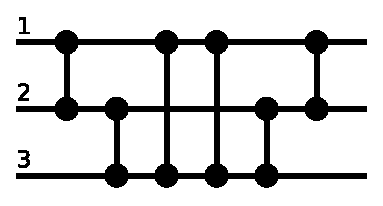
\includegraphics[width=0.4\textwidth]{gates1}
  \hfill
  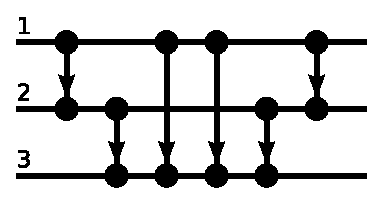
\includegraphics[width=0.4\textwidth]{gates2}
  \caption{Quantum Circuits.
  On the left the gates are represented by two-body symmetric interactions of
  the type XX+YY.
  On the right the symmetry is broken with with asymmetric interactions of the
  type XY-YX.}
  \label{fig:qcircuit}
\end{figure}

In the top left plot in Fig.~\ref{fig:init1},
the gates of Fig.~\ref{fig:qcircuit} acts on the network with the symmetric
Hamiltonian in eq.~\ref{eq:HS}.
The probability of finding the excitation in node two or three is bounded to
some value below 0.6.
In the top right plot the time reversed Hamiltonian
$H'=R_{z1}(\pi)HR_{z1}(\pi)$~is used and shows exactly the same
probabilities.

On the bottom an antisymmetric Hamiltonian (see eq.~\ref{eq:HA}) is used. 
The antisymmetric interaction is given by the initial symmetric Hamiltonian
where the first spin is rotated by $\pi/2$.
In this case the probabilities of encountering the excitation on node two or
three reach almost one.
Moreover the time symmetry is broken as shown by the fourth panel.

\yo{I would suggest a picture (related to Fig.~\ref{fig:init1}), or an animation,
for a transition diagram between 3 states
(i.e. 3 points, 6 directed arrows with probabilities).
It would make explicit how does probability "circulate". }

\begin{figure}[p]
  \centering
  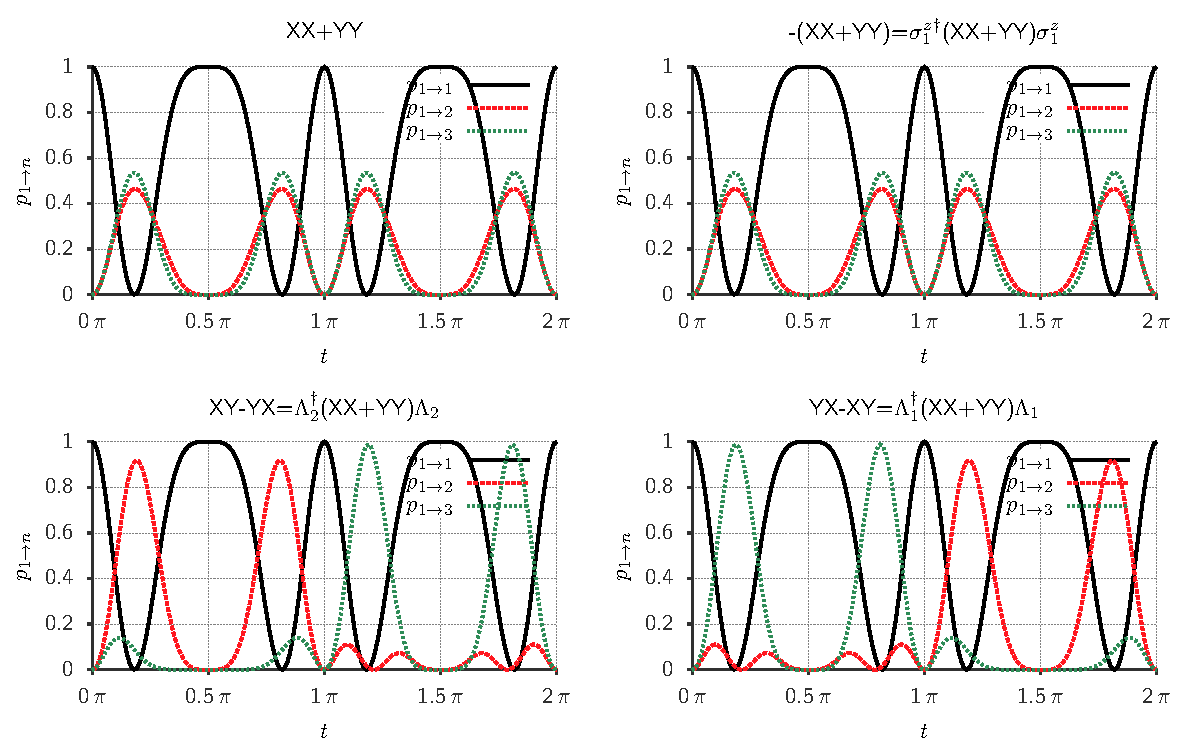
\includegraphics[width=0.8\textwidth]{3qbit_001}
  \caption{Breaking time symmetry.
  The initial state is represented by an excitation on qubit one. The
  occupation probability of qubit $n$ ($p_{1\to n}$) is depicted for different
  type of gates.
  On the top the interaction is symmetric $H=\frac 12 (XX+YY)$. The time inverse
  evolution is simulated rotating the first qubit with $\sigma_z$. The two
  evolutions match.
  The plots on the bottom represent antisymmetric gates $H=XY-YX$. In this
  case the time reversed evolution does not match the positive time one.
  Moreover, breaking time symmetry allows to direct the excitation
  toward the other nodes of the network, reaching an occupation of almost one.
  Here $\Lambda_n$ is the $2\times2$ diagonal matrix with entries 1 and $i$
  acting on the wire $n$.
  }
  \label{fig:init1}
\end{figure}



\begin{figure}[p]
	\begin{center}
		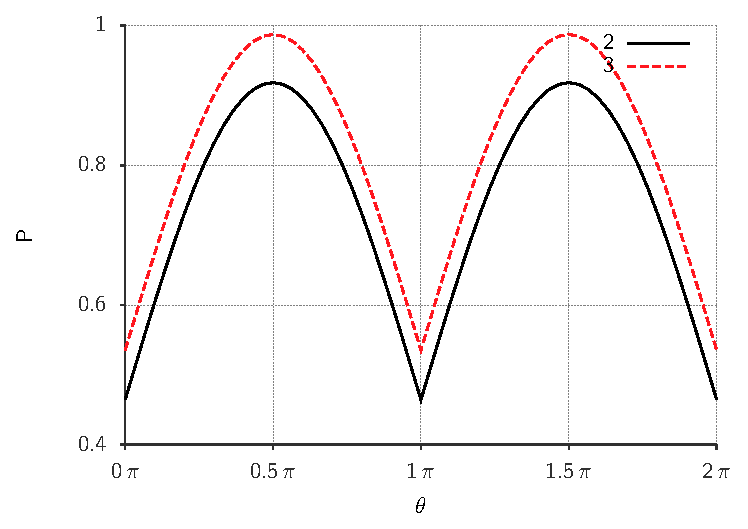
\includegraphics{opt-time}
	\end{center}
	\caption{Optimized Transport for the unitary family $U(\theta)$.
	The plot shows the best value of the transport from site one to site two
	(black solid line) and to site three (red dashed line), optimized on $t$.}
	\label{fig:opt}
\end{figure}


In Fig.~\ref{fig:init23} the same evolution, with the same gates are shown for
initial states localized on qubit two or three.


\begin{figure}[p]
  \centering
  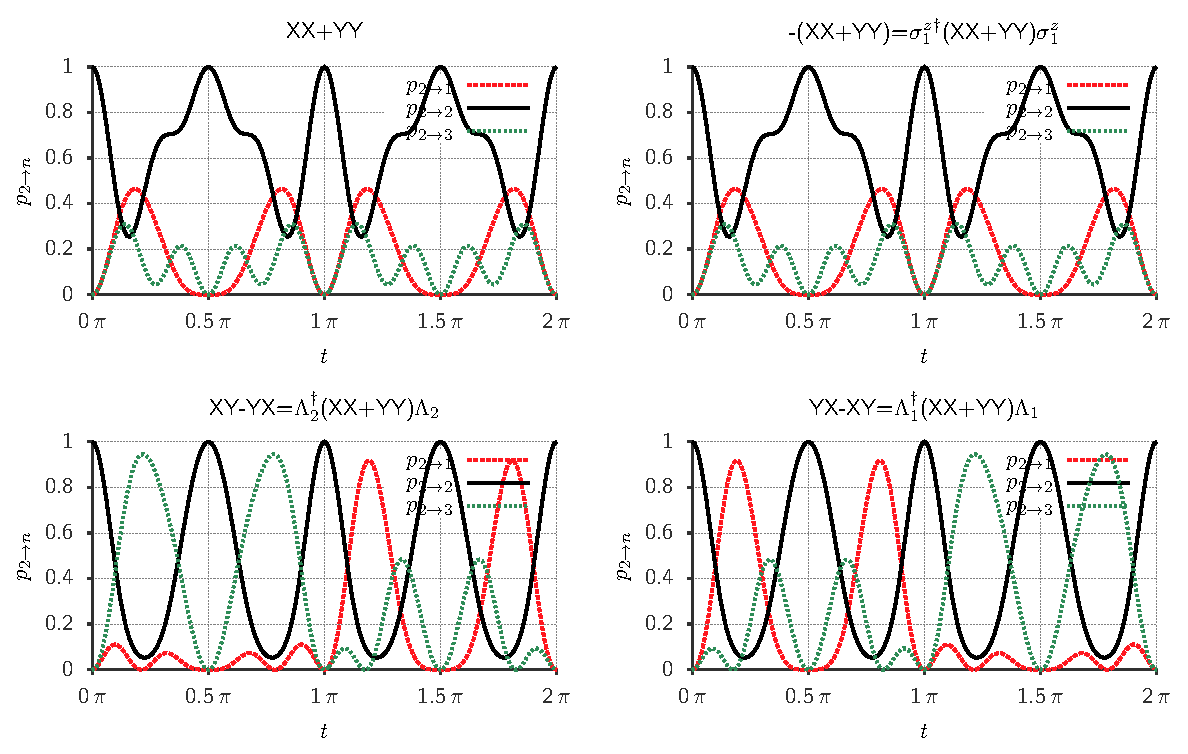
\includegraphics[width=0.8\textwidth]{3qbit_010}\\
  \vskip 10pt
  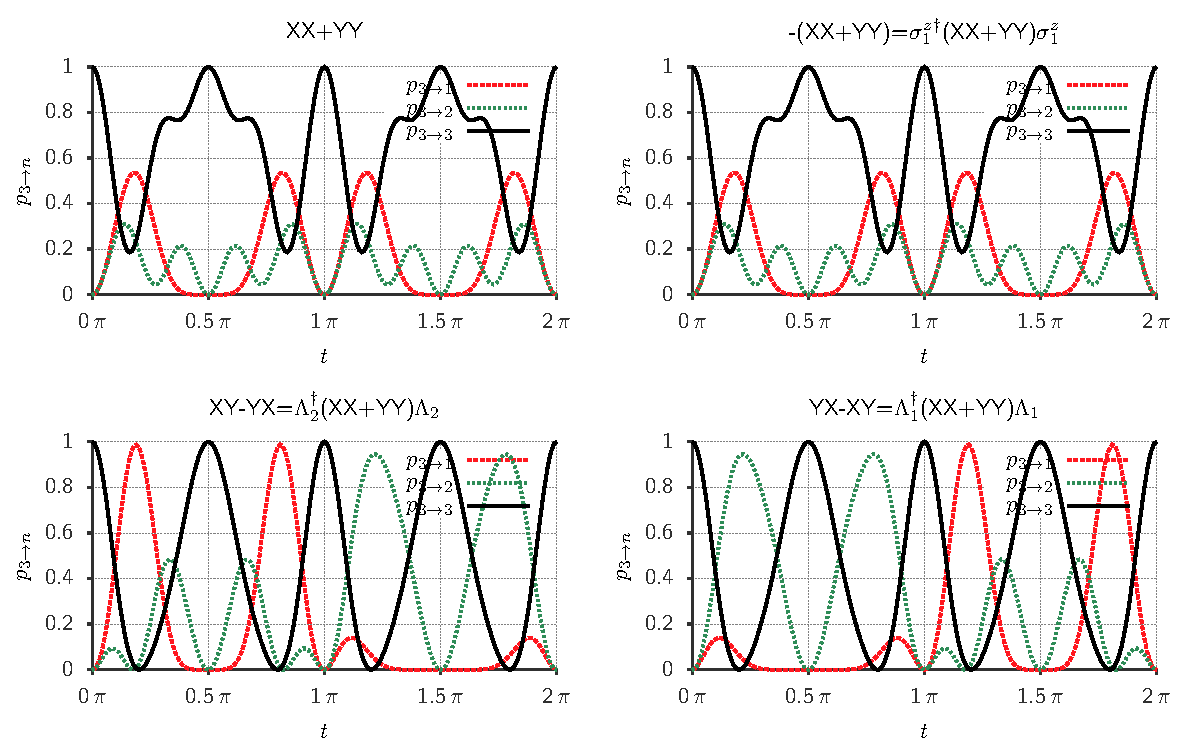
\includegraphics[width=0.8\textwidth]{3qbit_100}
  \caption{Here the initial state is localized on node two or three.}
  \label{fig:init23}
\end{figure}

\section{Connection to matchgates} 

The so called matchgates represent a family of quantum circuits which have been 
well studied in the literature, see e.g.~\cite{JM08, RFSW10}.  The general parameterized match gate is defined as 
\begin{align}
\notag
M_{AB} &:= 
\begin{pmatrix}
a_{11} & & & a_{12}\\
& b_{11} & b_{12} \\
& b_{21} & b_{22} \\
a_{21} & & & a_{22}
\end{pmatrix}
\end{align}
Such that the matrix $A$ ($B$) with entries $a_{ij}$ ($b_{ij}$) are $U(2,\CC)$ matrices with the same determinant.  

We recall now the general definition of the gates we consider here 
\begin{align}
\notag
R_z(\phi)e^{-i\theta(XX+YY)}R^\dagger_z(\phi) &= e^{-i \theta[\cos\phi(XX+YY)+\sin\phi(XY-YX)] }
= 
\begin{pmatrix}
1\\
& \cos(\theta) &  -ie^{-i\phi}\sin(\theta)\\
& -ie^{i\phi}\sin(\theta) & \cos(\theta)\\
& & & 1
\end{pmatrix}
\end{align}
In which case $\det A=\det\I=1$ and $\det B = \cos^2\phi + \sin^2\phi =1$ and so for all real values of $\theta$, $\phi$ this gate is indeed a match gate. 

In \cite{RFSW10} the authors present a general factorization for the parameterized matchgate. An immediate consequence of the fact that our gate family is a sub-class of the matchgates is that we could use the gate factorization in \cite{RFSW10} for a circuit realization, though alternative constructions are also possible. 




\section{Questions}

\begin{enumerate} 
\item other ideas?   
\end{enumerate} 



\appendix
\section{Mathematical background}

We are concerned with finite-dimensional quantum mechanics here. It is
assumed the reader is familiar with this standard mathematical
scenario, described in for instance reference \cite{s}.

\begin{definition}[Antilinear operators]
An \emph{antilinear} operator~$A: X \to Y$
(where $X$ and $Y$ are complex vector spaces) fulfills
\be
A(a x +b y) = \overline{a} Ax +\overline{b}Ay
\ee
for every $x,y \in X$, $a,b \in \CC$.
The product of a linear and an antilinear operator is antilinear, and
the product of two antilinear operators is again linear.

The \emph{adjoint}~$A^\dagger: Y \to X$ of an antilinear operator $A$
(with respect to an inner product $\iprod{\cdot}{\cdot}$)
is defined slightly differently from the adjoint of a linear operator, involving an
additional complex conjugation:
\be
\iprod{y}{Ax} = \overline{\iprod{A^\dagger y}{x}} \quad \forall x \in X, y \in Y.
\ee
This results in awkwardness when using the Dirac notation. Properties of antilinear operators include:
\begin{itemize}
\item
If $A$ is antilinear then so is~$A^\dagger$.

\item
Just like with linear operators, we
have~$(A^\dagger)^\dagger = A$.

\item
For any combination of linear and antilinear operators, we
have~$(AB)^\dagger = B^\dagger A^\dagger$.

\item
Apparently the trace of an antilinear operator is ill-defined (cannot
be made basis-independent?).
For $A, B$ linear we have\footnote{General basis expansion: If $\{k_i\}_i$ is an orthonormal basis for~$X$, we have
  $x = \sum_i \iprod{k_i}{x}k_i$ for any~$x \in X$.}
\begin{align}
\notag
\Tr(AB)
&:= \sum_k \iprod{k}{ABk}
= \sum_{km} \iprod{k}{A \iprod{m}{Bk}m}
= \sum_{km} \iprod{m}{Bk} \iprod{k}{Am}\\
&= \sum_{km} \iprod{m}{B\iprod{k}{Am}k}
= \sum_{m} \iprod{m}{BAm}
= \Tr(BA).
\end{align}
For $A, B$ \emph{both} antilinear (so $AB$ is linear, and trace again defined) we get
\begin{align}
\notag
\Tr(AB)
&= \sum_k \iprod{k}{ABk}
= \sum_{km} \iprod{k}{A \iprod{m}{Bk}m}
= \sum_{km} \overline{\iprod{m}{Bk}} \iprod{k}{Am}
= \sum_{km} \iprod{Bk}{m} \iprod{k}{Am}\\
&= \sum_{km} \iprod{\overline{\iprod{k}{Am}} Bk}{m}
= \sum_{km} \iprod{B \iprod{k}{Am}k}{m}
= \sum_{m} \iprod{B Am}{m}
= \overline{\Tr(BA)}.
\end{align}

\item
\todo{What about the associativity of antilinear ops???}
\end{itemize}
\end{definition}

\begin{definition}[Antiunitary operators]
An invertible antilinear operator~$W: X \to X$ is called
\emph{antiunitary} iff
\be
\iprod{Ax}{Ay} = \overline{\iprod{x}{y}} \quad \forall x, y \in X.
\ee
This yields
\be
\iprod{x}{y} = \overline{\iprod{Ax}{Ay}} = \iprod{A^\dagger A x}{y}
\quad \forall x, y \in X,
\ee
and thus~$A^\dagger A = \I$. Since $A$ is invertible we must
have~$A^{-1} = A^\dagger$, just like with unitary operators.
\end{definition}

\begin{definition}[Complex conjugation operator]
Given a basis~$\{\ket{B_k}\}_k$, complex conjugation of the coefficients of any
given vector $\ket{\psi} = \sum_k a_k \ket{B_k}$
in this basis can be represented as an antilinear operator $K_B$, such that  
\be
K_B \ket{\psi} := K_B \sum_k a_k \ket{B_k}
= \sum_k \overline{a_k} \ket{B_k}.
\ee
We have~$K_B^{-1} = K_B^\dagger = K_B$, and thus $K_B$ is antiunitary.

If we have two bases related by the unitary operator~$U$,
such that~$\ket{C_k} = U \ket{B_k}$, we have
\be
K_C \left(\sum_m v_m \ket{C_m} \right)
= \sum_m \overline{v_m} \ket{C_m}
= U \left(\sum_m \overline{v_m} \ket{B_m} \right)
= U K_B \left(\sum_m v_m \ket{B_m} \right)
= U K_B U^{\dagger} \left(\sum_m v_m \ket{C_m} \right),
\ee
and thus
\be
K_C = U K_B U^{\dagger}.
\ee
\end{definition}

\begin{definition}[Representation of antilinear operators]
Any antilinear operator~$A$ can be represented using~$K_B$ and a
linear operator~$L_B$ as
$A = L_B K_B$,
so that $A$ and $L_B$ have the same matrix elements in the basis~$B$.
If we require $A = L_B K_B = L_C K_C$, we obtain
\be
L_C = 
A K_C = L_B K_B K_C = L_B K_B U K_B U^{\dagger}
= L_B \overline{U} U^\dagger,
\ee
where the complex conjugation is in the basis~$B$.
Hence the choice of the basis has no inherent importance.
\end{definition}

\begin{example}[Odd example]
You cannot simply operate with $T$ towards the left as usual!
Either only operate towards the right (minding complex factors which
you have to conjugate), or use the definition of the adjoint.
\be
(TUT)_{ab} = \bra{a}TUT\ket{b} = \bra{a}TU\ket{b}
= \sum_x \bra{a} T \ketbra{x}{x} U\ket{b}
= \sum_x \bra{a} T \ket{x} U_{xb}
= \sum_x \braket{a}{x} \overline{U_{xb}}
= \overline{U}_{ab}.
\ee
This matrix property justifies our somewhat sloppy
notation~$\overline{U} := TUT$.
\end{example}


\section{Time symmetry in general}

\subsection{Definition}
Generally I think time symmetry means this: We have an antiunitary
operator~$T$ which, to quote Ballentine, \emph{does not reverse the direction of time},
but instead \emph{reverses the direction of motion} of a physical system.

In a system composed of particles (maybe with spin), the effect of~$T$
on every particle is the following:
\begin{align}
T\vec{Q}T^{-1} &= \vec{Q},\\
T\vec{P}T^{-1} &= -\vec{P},\\
T\vec{S}T^{-1} &= -\vec{S},
\end{align}
where~$\vec{Q}, \vec{P}$ and $\vec{S}$ are the position, momentum and
spin operators, respectively.
$T$~thus reverses spins and momenta, but preserves the positions.
Orbital angular momentum is also reversed, since
$\vec{L} = \vec{Q} \times \vec{P}$, and consequently so is the total
angular momentum~$\vec{J} = \vec{L} + \vec{S}$.

The main idea is this: You suddenly reverse the direction of the
momentum and spin of every particle in the system. Will the system now
evolve \emph{as if} it were moving backwards in time? Can you reverse
the arrow of time like this? In a $T$-symmetric system the answer is yes.
In other words, the system is said to be $T$-symmetric iff
\be
T^{-1} U(t) T U(t) = \I \quad \forall t.
\ee
\todo{Add an arbitrary global phase?}
Equivalently we should have~$T U(t) T^{-1} = U^\dagger(t)$.

If $U$ is generated by a time-independent Hamiltonian~$H$, we obtain
\be
T U(t) T^{-1} 
= T e^{-i H t/\hbar} T^{-1} 
= e^{i THT^{-1} t/\hbar}  
= U^\dagger(t)
= e^{i H t/\hbar} \quad \forall t.
\ee
as the condition for~$T$ symmetry. Now Stone's theorem on
one-parameter unitary groups says this is equivalent to
\be
T H T^{-1} = H.
\ee



\subsection{T symmetry for spins}

For spins, the~$T$ operator is given by
\be
T := R_y(\pi) K = e^{-i \pi S_y/\hbar} K,
\ee
where~$K$ is complex conjugation in the standard basis (where~$S_z$ is
real and diagonal, $S_x$ real and $S_y$ purely imaginary).
Both $K$ and $R_y$ are basis-dependent, but the dependencies cancel and
one always obtains~$T S_k T^{-1} = -S_k$.
See Ballentine p.~382.




\subsection{Transition amplitudes}
For any two states $\ket{\psi_i}$, $\ket{\psi_f}$ (not just basis
states) and a $T$-symmetric propagator~$U$, we have
\be
\bra{\psi_f} U \ket{\psi_i}
= \bra{\psi_f} T^\dagger U^\dagger T \ket{\psi_i}
= \iprod{\psi_f}{T^\dagger U^\dagger T \psi_i}
= \overline{\iprod{U T \psi_f}{T \psi_i}}
= \iprod{T \psi_i}{U T \psi_f}
= \bra{T \psi_i} U \ket{T \psi_f}.
\ee




\section{Sign-reversing a Hamiltonian}

Instead of T-transforming the propagator (or the states) to go ``back
in time'', we can also similarity transform the Hamiltonian so
that it is sign-reversed. This only works for some Hamiltonians, however.

The eigenvalue spectrum of an operator~$H$ is not changed by a similarity transform~$S$:
\be
\sigma(H) = \sigma(S H S^{-1}) \quad \forall H, S.
\ee
In order to be able to negate an operator (a Hamiltonian, for example)
using a similarity transform (any, not just a local one), $S H S^{-1} = -H$, we must have
\be
\sigma(H) = \sigma(S H S^{-1}) = \sigma(-H) = -\sigma(H).
\ee
This is fulfilled by all two-spin XY Hamiltonians, but not by a
fully connected 3-spin $H_S$ network, for example.


\section{Random unfinished stuff}

\subsection{Representations of the Hamiltonian} 
There exists two projectors taking a matrix $H$ to its symmetric and antisymmetric parts, respectively given as.  
$$
P_{sym}(H) = \frac{H+H^\top}{2}
$$ 
$$
P_{asym}(H) = \frac{H-H^\top}{2}
$$ 

Write the matrix $H$ in terms of a symmetric ($S$) and antisymmetric ($A$) part as 
$$ 
H = S + A
$$ 
and further assume that $H = H^\dagger$.  Then 
$$ 
S + A = S^\dagger + A^\dagger, 
$$ 
where the sum ($+$) could be replaced by the direct sum ($\oplus$). 
Yet since $S^\top = S$ and $A^\top = - A$ by assumption, we must have that $S$ is purely real, and $A$ is purely imaginary.  
We then will abuse notation slightly and write $A$ as $iA$ and $H$ as 
$$ 
H = S + i A
$$ 
which is equal to its own conjugate transpose.  We then have a general expression for a Hamiltonian $H$.  Under the complex image of the exponential map we have 
$$ 
e^{t(A-iS)} 
$$ 
and then the dagger ($\dagger$) acts as transposition on $A$ ($A^\dagger =
A^\top = - A$) and as conjugation on $iS$ ($[iS]^\dagger =
\bar{i}\overline{S^\top} = \bar{i}S = - iS$). 

If $\| P_{sym}(H)\| = \| P_{asym}(H)\|=0$ the
process has no time dependence so is invariant under time inversion. We can go
slightly further and state that: 

\begin{remark}[Necessity of non-vanishing antisymmetric projector]
It is necessary that $\| P_{asym}(H)\|$ is non-vanishing to
break time-inversion symmetry.  If $\| P_{asym}(H)\| = 0$ this
implies in particular that $H = P_{sym}(H) = S$ and so $H = \bar H$ and hence
the corresponding evolution is time-symmetric.  Furthermore, here the dagger
reduces to element wise, complex conjugation of the corresponding propagator.  
\end{remark}




\begin{remark} 
It's a matter of perspective which of the terms in $H=S+iA$ is the complex factor: the traditional symmetric transaction terms, are purely imaginary in $e^{t(A-iS)}$, whereas the anti-symmetric terms which could break TS are purely real.  This becomes particularly evident when considering the definition of the transition probability: 
$$ 
|\bra{f}e^{-itH}\ket{s}|^2 = |\bra{f}Te^{-itH}T\ket{s}|^2
$$ 
Again writing $H = iA + S$ and introducing the notation $H_\pm = iA \pm S$ we see that 
$$ 
|\bra{f}e^{-itS+tA}\ket{s}|^2 = |\bra{f}e^{itS+tA}\ket{s}|^2
$$ 
and so we conclude that the transition rates induced by $H_-$ are identical to those induced by $H_+$.  Whenever $2A=H-H^\top$ is vanishing, one recovers the anticipated time-symmetric case. 
\end{remark} 

%\begin{remark}[Commutation relations]
%$$
%[H, E]=0
%$$ 
%and for purely antisymmetric $H$ we have 
%$$ 
%\{H, E\}=0
%$$ 
%More generally we have that 
%$$ 
%[H,E]=[S+iA, E] = i[A,E]=2iAE=iE(H^\top-H) 
%$$ 
%\end{remark}

\subsection{Specfic properties of breaking time-symmetry} 

In this section we are concerned with circuits formed from the gates $U=U^\top$ generated by the symmetric Hamiltonian.  
$U=U^\top \implies \text{TS}$, so $U\neq U^\top$ is a necessary but
not sufficient condition for breaking time symmetry.  
%\begin{enumerate}
%\item $\neg[U=U^\top]$ $\wedge$ $\neg \text{TS}$ is possible 
%\item $\neg [U=U^\top]$ $\implies$ $\text{TS}$ is possible 
%\item $[U=U^\top]$ $\implies$ $\neg \text{TS}$ is not possible 
%\item $[U=U^\top]$ $\implies$ $\text{TS}$ is possible, as already stated 
%\end{enumerate} 

More on necessary conditions:
For a process to be not TS, we must have
\be
U^\top \neq U~\text{and also that}~U^\dagger \neq U 
\ee
However, the special case $U = \bar U$ is allowed.

\begin{remark}[General case: mixed symmetry] 
We note that in the general case
when both $H+H^\top$ and $H-H^\top$ are non-vanishing,
\be
U^\dagger = e^{t (A -i S)^\dagger} = e^{t (A^\top +i S^\top)} = e^{t(-A +iS)},
\ee
and the dagger operation requires both transposition and complex conjugation.
\end{remark} 

\begin{remark}[$U = \bar U$] 
From this we note that $U = \bar U \Leftarrow H = iA$ for $H$
the corresponding Hamiltonian and $A$ such that $A^\top = -A$.  This
corresponds to the purely antisymmetric case, and the orthogonal group
of matrices.
\end{remark} 

\begin{lemma}\label{lemma:complex} 
Given unitary $U=\bar U$, and eigenvector $\ket{\psi}$ such that $e^{-i \lambda}$ is the corresponding eigenvalue, than $T\ket{\psi}$ is necessarily an eigenvector with eigenvalue $e^{i \lambda}$. 
\end{lemma} 
\begin{proof} 
We are given $\ket{\psi}$ such that 
$$ 
U\ket{\psi} = e^{-i \lambda}\ket{\psi}
$$ 
From this we have 
$$ 
T(U\ket{\psi}) = (TUT)(T\ket{\psi} )= e^{i \lambda}T \ket{\psi} 
$$  
but $TUT = U$ by assumption so $T \ket{\psi}$ is an eigenvector of $U$ with eigenvalue $e^{i \lambda}$. 

\end{proof} 


\bibliography{chiral-bib}

\end{document}

 
